% Load the kaobook class
\documentclass[
	fontsize=10pt, % Base font size
	twoside=false, % Use different layouts for even and odd pages (in particular, if twoside=true, the margin column will be always on the outside)
	%open=any, % If twoside=true, uncomment this to force new chapters to start on any page, not only on right (odd) pages
	secnumdepth=1, % How deep to number headings. Defaults to 1 (sections)
]{kaobook}

% Choose the language
\usepackage[english]{babel} % Load characters and hyphenation
\usepackage[english=american]{csquotes}	% English quotes

% Load packages for testing
\usepackage{blindtext}
%\usepackage{showframe} % Uncomment to show boxes around the text area, margin, header and footer
%\usepackage{showlabels} % Uncomment to output the content of \label commands to the document where they are used

% Load the bibliography package
\usepackage{kaobiblio}
\addbibresource{intro-pubinv.bib} % Bibliography file

% Load mathematical packages for theorems and related environments
\usepackage{kaotheorems}

% Load the package for hyperreferences
\usepackage{kaorefs}


\graphicspath{{images/}{./}} % Paths where images are looked for

\makeindex[columns=3, title=Alphabetical Index, intoc] % Make LaTeX produce the files required to compile the index


\begin{document}

%----------------------------------------------------------------------------------------
%	BOOK INFORMATION
%----------------------------------------------------------------------------------------

\titlehead{Public Invention}
\title[Public Invention]{Public Invention}
\author[RLR]{Robert L. Read}
\date{\today}
\publishers{Public Invention, a US public charity}

%----------------------------------------------------------------------------------------

\frontmatter % Denotes the start of the pre-document content, uses roman numerals

%----------------------------------------------------------------------------------------
%	COPYRIGHT PAGE
%----------------------------------------------------------------------------------------

\makeatletter
\uppertitleback{\@titlehead} % Header

\lowertitleback{
	\textbf{Disclaimer} \\
	You can edit this page to suit your needs. For instance, here we have a no copyright statement, a colophon and some other information. This page is based on the corresponding page of Ken Arroyo Ohori's thesis, with minimal changes.

	\medskip

	\textbf{Copyright 2021, Robert L. Read} \\
%%	\cczero\

	\medskip

	\textbf{Colophon} \\
	This document was typeset with the help of \href{https://sourceforge.net/projects/koma-script/}{\KOMAScript} and \href{https://www.latex-project.org/}{\LaTeX} using the \href{https://github.com/fmarotta/kaobook/}{kaobook} class.

	\medskip

	\textbf{Publisher} \\
	This book has not yet been printed. \@publishers
}
\makeatother

%----------------------------------------------------------------------------------------
%	DEDICATION
%----------------------------------------------------------------------------------------

\dedication{
  If you want to build a ship, don’t drum up the men to gather wood, divide the work, and give orders. Instead, teach them to yearn for the vast and endless sea.\\
  \flushright -- Antoine de Saint-Exupéry
  \\
  The chances of your success are zero, but the importance is infinite; therefore, I support you.\\
  \flushright -- Sir W. Lawrence Bragg

}

%----------------------------------------------------------------------------------------
%	OUTPUT TITLE PAGE AND PREVIOUS
%----------------------------------------------------------------------------------------

% Note that \maketitle outputs the pages before here
\maketitle

%----------------------------------------------------------------------------------------
%	PREFACE
%----------------------------------------------------------------------------------------

\chapter*{Preface}

This is a draft work whose purpose is explain and promote Public Invention as a
movement and philosophy. My hope is to create a coherent and convincing work.
This work will likely be published electronically by Public Invention (the organization),
but we will also seek a print-publisher who is willing to keep the work open access.

-- Robert L. Read

%----------------------------------------------------------------------------------------
%	TABLE OF CONTENTS & LIST OF FIGURES/TABLES
%----------------------------------------------------------------------------------------

\begingroup % Local scope for the following commands

% Define the style for the TOC, LOF, and LOT
%\setstretch{1} % Uncomment to modify line spacing in the ToC
%\hypersetup{linkcolor=blue} % Uncomment to set the colour of links in the ToC
\setlength{\textheight}{230\vscale} % Manually adjust the height of the ToC pages

% Turn on compatibility mode for the etoc package
\etocstandarddisplaystyle % "toc display" as if etoc was not loaded
\etocstandardlines % "toc lines as if etoc was not loaded

\tableofcontents % Output the table of contents

\listoffigures % Output the list of figures

% Comment both of the following lines to have the LOF and the LOT on different pages
\let\cleardoublepage\bigskip
\let\clearpage\bigskip

\listoftables % Output the list of tables

\endgroup

%----------------------------------------------------------------------------------------
%	MAIN BODY
%----------------------------------------------------------------------------------------

\mainmatter % Denotes the start of the main document content, resets page numbering and uses arabic numbers
\setchapterstyle{kao} % Choose the default chapter heading style

\pagelayout{wide} % No margins
\addpart{The Joy of Public Invention}
\pagelayout{margin} % Restore margins

\chapter{“Invent in the public, for the Public.”}


Benjamin Franklin (1705-1790) did not patent the Franklin stove because
he believed it to be too useful an invention to legally encumber.
Benjamin Franklin has been
called ``The First American''\cite{Brands2000}, but I think of him as the
first Public Inventor.
If you read the autobiography of Nikola Tesla (1856-1943)
``My Inventions''\cite{Tesla1982},
you discover a devout public servant
(in a non-denominational sense), who certainly wanted to make
money but whose deepest motivation was to see human progress.
R. Buckminster Fuller (1895-1983) wrote extensively on the act of invention
as a moral act: nerve gas is bad, vaccines are good\cite{Fuller1981}.
Richard Stallman (1953-) articulated the principles of free software
and in so doing indirectly increased the wealth and well-being
of the planet tremendsouly\cite{Stallman2002free}.
This book is my attempt to extend and promote the work of
those inventors to create a stronger movement which we could
call Public Invention.

\nocite{laurel2001}

Invention is the most spectacular way to advance human progress.
It is odd that our politicians mostly ignore it.
The story of human history is largely a story of technological
advance careening foward from the stone age with
a speed which is inexorably, and frightentingly, building,
perhaps to a climax.
Those who believe it will end in a dark and terrible
destruction are not fools;
but that fate is not certain.
We as a planet can choose instead to build a bright future
in which humanity explores the universe together in peace.
This will happen only if we understand technology as the
powerful moral force that it is.

For the last 100 years, technological advance has been driven
by two engines: profit and academic research.
The modern emphasis of Universities of patenting research
and the governmental practice of subsidizing research which
is monopolized by for-profit firms has blurred the distinction.
Nations have long recognized the value of technology for
competiting with other nations via
war or mercantilism. Public Invention hopes to be a movement
that does not replace for-profit research and academic research,
but becomes a third engine. The motto of Public Invention
is ``Invent in the public, for the Public.''

\begin{marginfigure}[-5.5cm]
    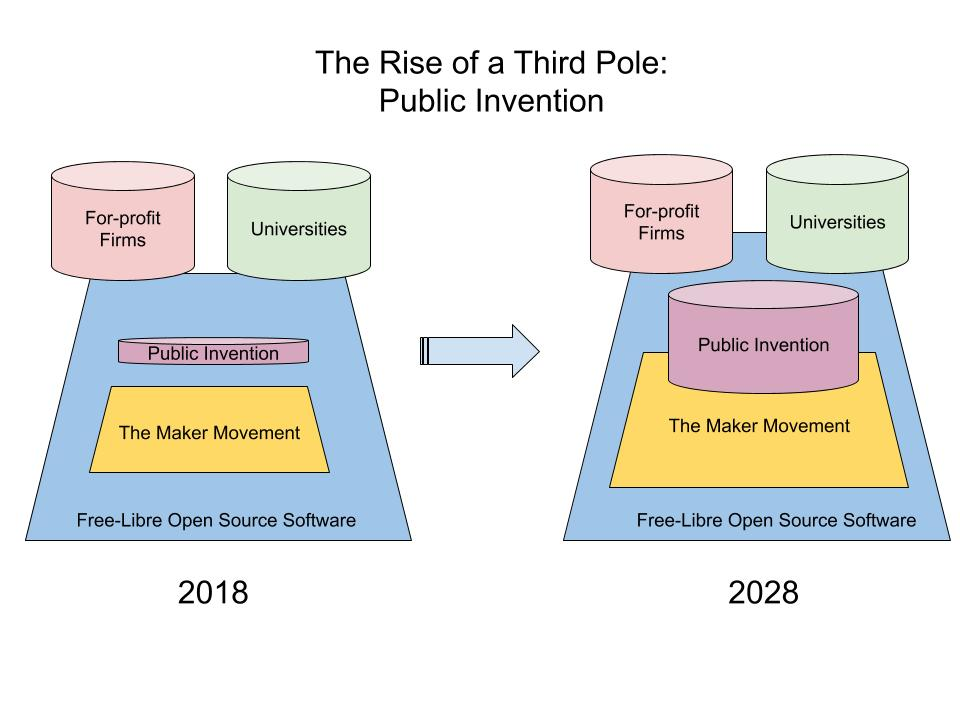
\includegraphics{figures/The_Rise_of_Public_Invention.jpg}
  \caption{The Rise of Public Invention as a Third Pole of Progress}
  \labfig{rise}
\end{marginfigure}

This means the Public Inventor does not seek monopolies in
the form of patents or other intellectual property but
gives an invention freely to the whole world without prejudice.
Anyone is free to use the invention, including for the purpose
of making a profit, but nobody is giving the privilege of
exclusive rights to it.

Buckminster Fuller made a clear distinction between what he
called ``killingry'', or weapons, and ``livingry''--that
which increase the good in the world. The Public Inventor
must not build weapons. This is impossible
to do perfectly.
Even a pillow can be used as a weapon. Nonetheless,
technologists are not relieved of the duty to invent
good things instead of bad things just because it is
intellectually difficult to decide what is good and what is bad.
The Public Inventor accepts this burden as does the best they can.

Benjamin Franklin said, ``We must, indeed, all hang together or,
most assuredly, we shall all hang separately.''
His wit was poignant because he meant the American revolutionary
leaders would indeed have swung from a British rope for treason
if the Revolutionary war had been lost.
But in 2021 his words still ring true. Buckminster Fuller
believed that humanity would either destroy itself or
have a bright, Star Trek-like future---there is no
middle ground.
We cannot continue to muddle along
taking weak action on global warming.
The COVID-19 pandemic has shown that we are all connected
in a most intimate way, whether we like it or not.
A disease incubated in my body may kill you, and vice versa.
Therefore the Public Inventor must at some level seek
the wealth and well-being of the whole world.
Narrow national chauvinism is no longer a useful or profitable
behavior.

We could define Public Invention simply as invention in the
public interest.
In that sense, it is closely related to humanitarian engineering.
Humantarian engineering requires a great deal of problem-solving,
innovation, and ingenuity. The distinction is that ``invention''
means something truly novel which has never existed before.
Public  invention values the truly novel, whereas
humanitarian engineering values the truly useful.

In the future, it will be common place for people to move freely
between
the three engines of for-profit firms, academic research,
and public invention.
Public invention will not replace the other two engines,
but augment them.
Public invention is a moral act, but it is not a moral duty.
Some people will want to be public inventors some of the time.

\chapter{The Arc of Progress}

It is easier to be a motivated public inventor
if one sees oneself as a minor character in a great story,
the greatest story that we can know, the story of human progress.\marginnote{``You can be the captain, and I will draw the chart..." -- Rush, Closer to the Heart.}
It does not particular matter if you believe this progress
is positive or negative, though Steven Pinker is has argued overwhelmingly it
is astoundingly positive. \cite{Pinker2019}
It doesn't matter if you see it as rooted in
Babylonia, ancient Rome, Jerusalem, the Chin dynasty, the
Enlightenment, or the American Revolution.
The more history you know, the better, of course.
But being part of a great story gives your actions meaning.
It is impossible to measure out your life in coffee spoons
if you see yourself as part of a great story.

Much science fiction is dystopian and dark, but almost all
of it sees humanity placed in the arc of some greater story,
in which the characters are agents.
This is not as common in fantasy, but it is true of the
greatest fantasy.
Certainly, the Marvel Cinematic Universe, the Lord of the Rings,
Star Wars, Dune, the Space Trilogy of C.S. Lewis,
and the Chronicles of Narnia all accomplish this.
Distressingly, the idea of the arc of human progress is
less present in political statments\marginnote{I dare not say political discourse, which disappeared when Newt Gingrich turned the
Republican party against compromise.}
than it was in my youth.
Without a sense of where we have been and where we are going,
politics misses the point, and becomes mere tribal bickering.\marginnote{Richard Nixon spoke of population growth and control}

\chapter{The Joy of Public Invention}

Public invention takes the joy of invention and multiplies
it by the joy of helping others.
Making something truly new is a roller coaster ride
of emotions.
The inventor is frought with doubts.
Is the invention even possible?
Has someone done this earlier?
Am I too stupid to accomplish this?
Often a new idea creates innumerable frustrations.
The expensive equipment breaks at a critical momemnt.
There may be collaborators,
but there are no experts to turn to, because by definition
the invention has never been made before.
Despite all of the doubts and frustrations, or
perhaps because of them, the eventual progress, if it
comes, is an intense joy.

Comic books and movies have taken a grain of truth
and mythologized out of proportion to create the trope
of the lone inventor.
Most invention is done by teams.
Math, is, in the end, always social.
The joy of collaboration is part of the attraction
of being a public inventor.

Each of us is unique and has unique gifts to bring
to the table.
In a sense this is true in any part of life,
but it is a especially true in the act of invention.
Each of us has a different voice, even if we sing
the same song.
However, by definition, invention is making something
not just new in the sense of a variation of something
old, however unique, but new in the sense of breaking new
ground.
An invention is not yet another rose, it is a new kind of flower.
Even mediocre inventors such as myself are essential and necessary.
The mediocre work makes the great work easier.

Some people have an invention inside them that has to get out.
The seed of an idea planted in childhood may mature in the unconscious
until the time is right for it emerge.
Sometimes this is because of a persons great love of something.
We have all seen people enchanting by flying or
infatuated with light.
Some people can spend years entranced by a math problem.
The inventions may be useful, but unprofitable.
Some may even be potentially harmful. Certainly many men,
including myself, are fascinated by shooting things at
high velocity, such as in guns or rockets or bows
or catapults or water guns.
So long as the invention is not designed to harm,
the invention should be allowed to be born.
The line between invention and art is sometimes blurred.
The public inventor should support whimsical inventions
when a person has a strong desire to make it.

The public inventor should not make fakes or toys.
That is, the public inventor should make an object
whose value is that it is a miniature version of some
other object or like some other object which has intrinsic value.
Making a model of a beautiful airplane or ship is valuable
and fun, but it is not invention.
Making a fake starship is not invention.

However, the desire to make something new even if the
utility of the invention is hard to define should be
respected. This may be because it is artful, or may
have nothing to do with art, and its value may lie
in some other dimension.
Often, an invention that wants to be made that has
no clear purpose is a forerunner of something else
which cannot be conceived until the first invention
is real and can be held in hand.

To me, public invention is really about love---love of humanity,
of beauty, of the planet, of math, and of my fellow-inventors.
For some of us, the joys of learning, collaboration, invention,
and helping the world melded together in public invention
is the greatest joy we can imagine.
At the end of my life my proudest acheivement will be my children,
and my second greatest sense of joy will come from the
inventions I have given the world, however small they may be.

\chapter{Why it makes more sense than in the past}

Participation in public invention makes more sense with
each passing decade.
Although we suffer from inequity, in raw terms the world
is more abundant than ever before.
Commodities are cheaper.
Fewer people live in poverty.
The number of people who are financially able to take
a few months out of the work force to work on a public invention
project without compensation is higher than ever.
People are more generous than ever before.
The number of people who make a substantial income
essentially through patronage and tipping is probably
hire than ever before.
In a world of abundance, the need to make a profit
or to work relentlessly at a career should
become less imperative.

In America today, housing in large cities
and formal education are exceptions
to the general trend of things becoming cheaper and easier to obtain.
Participating in public invention is a powerful way to
obtain two things provided by a formal education:
the learning and reputation.

There are specific technical reasons certain kinds of
public invention are far more accessible than ever before.
In the first place, the internet has made many tutorials
and how-to documents available almost for free, from
how to use a soldering iron to very sophisticated academic
papers.
Secondly, the free software movement has made an ocean
of high quality software available.
Although it takes effort, almost any computing task can
now be accomplished without paying a cent for software.
It remains the case that some of the best scientific tools
do not yet have free-gratis alternatives of similar quality,
but the trend is incontrovertible: the cost of computing
is getting cheaper.
I'm writing and typesetting this book right now
using mostly free software tools.
This same software generally also makes it cheaper to
build new software.
Usually, software that it free
as in free-pizza is free as in free-speech---meaning that
anyone has the freedom to use it as a starting point for making
something new.
Software has limitations, but it is extraordinarily versatile.
It is the most general-purpose of all technologies. The fact
that it is free is a fundamental enabler of public invention,
because capital attracted based on expectations of profits is
not needed.

Hardware is more expensive, but has gotten dramatically
more accessible at a low price. 3D printers that cost USD\$300
can now do astounding things that were not even possible 30
years ago. Similarly, it is now possible to design printed
circuit boards on free software and have them fabricated
and very low costs, usually in about two weeks.
This capability augments the old-fashioned but still
useful soldering iron as a means of making sturdy circuits.
Of course the reduction in the price of computers, which
includes single-chip micro-contollers used in electronic
embedded systems is legendary.

Although I am weak on bio-hacking, I believe the same
expansion of capability at reasonable cost has occurred in
the word of biology and biochemistry.
Even optics, in the form of microscopy and teloscopy,
has seen major improvements.

Batteris and solar power have enabled deployment of
electronics portably and to remote off-the-grid locations.
Significant improvements in cameras, sonar, and other
sensors have also increased the sophistication available
at low cost.

(Create Matrix/Infographic of relative acceleration in fields.)

Although hardware cost remain a relative imepdiment
(see Chapter \ref{chp:material} for Public Invention's policy),
the combination of cheap hardware, free software, and
cheap connectivity has made innovation and invention much easier.
Sharing and publication of inventions is a
critical part of public invention, and that is also
now easier than it has ever been.


\section{Makers into Public Inventors}

Makers know the joy of making.
The Maker movement supports creativity, skill building,
art, humor, and practical function.
Makers today, thanks in large part to Maker magazine
and Maker Faires, have thousands of fascinating
projects to prove from.
An invention has to be something novel
which has never been made before.
Making is not easy; it takes practice, problem solving, creativity,
and ingenuity, but usually not invention.
If the public invention movement had even ten per cent
of the energy of the maker movement, it would be a
tremndous force for good.

There is a natural progression from making to
public inventing which some makers will take.
This book is an attempt to create
for the Public Invention movement
a culture as strong and supportive as
Maker culture is today.


\chapter{The millifuller}


\begin{marginfigure}
  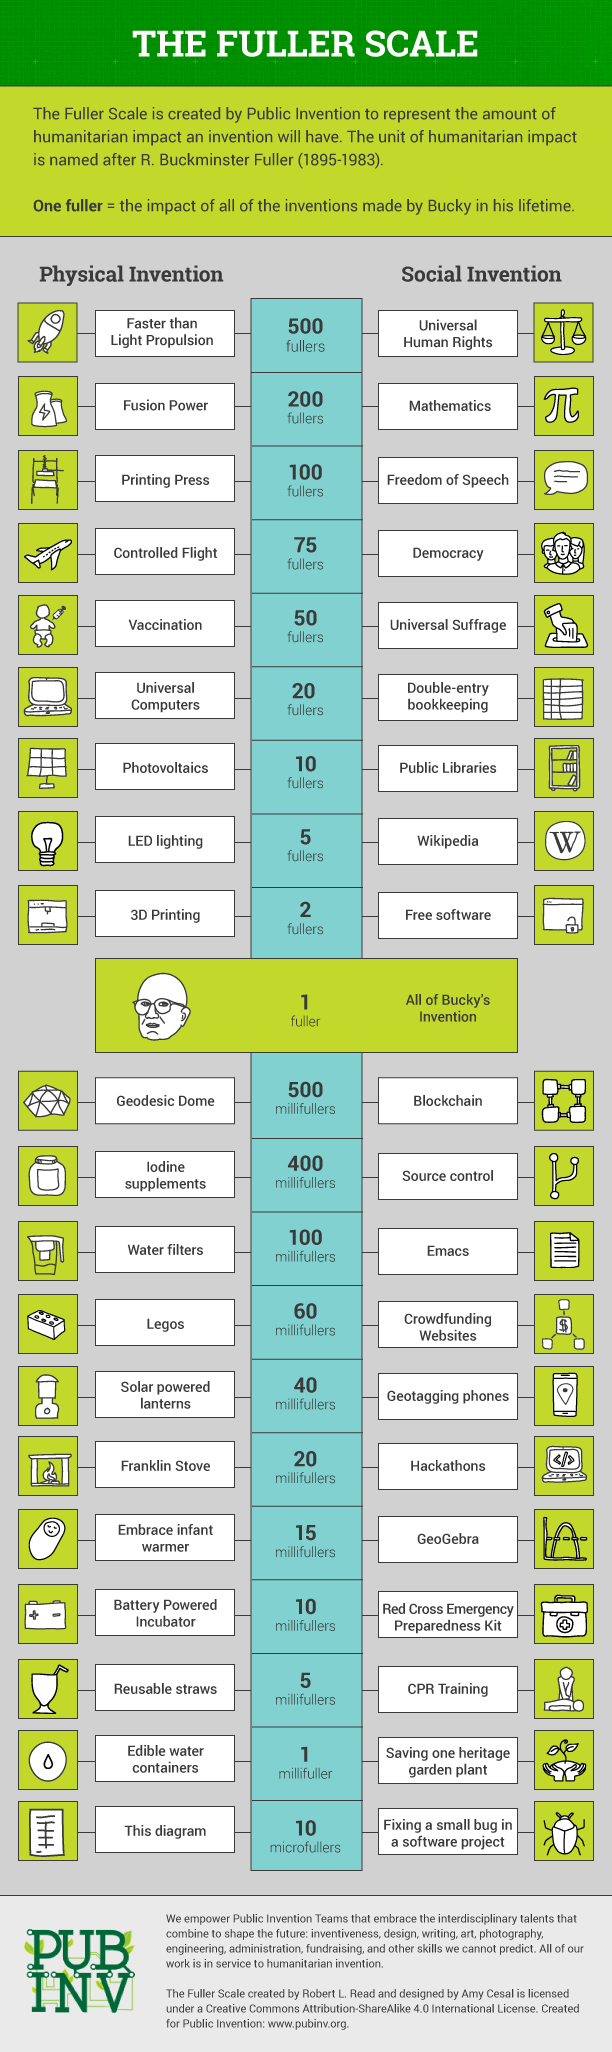
\includegraphics{figures/FullerScale.png}
  \caption{The Fuller Scale of Humanitarian Invention Value}
  \labfig{fullerscale}
\end{marginfigure}

Science is about truth; engineering is about compromise.

At Public Invention, we do both, but perhaps more engineering than
science.

Our goal is to have a large positive impact on many people; but time
and money are always in short supply.  How, then, to compromise on
which projects to prioritize?

In order to be able to even discuss the humanitarian impact of two
projects that may both need attention, it helps to be able to measure
humanitarian impact in some way. To do this, we have created “The
Fuller Scale“. The “fuller” is a new unit of humanitarian impact,
inspired by Buckminster Fuller, the great American champion of
invention as a moral good. It is by definition the impact of all of
the inventions of his long life.

It is, of course, subjective; the best things in life are.

A team of inventors does not need to agree perfectly to usefully
quantify impact. I hope in the future Public Inventors and other will
have conversations like:

“Well, I agree your robot technology is a useful search-and-rescue
idea. If it is worth 20 millifullers, then surely detecting
contaminated drinking water, which kills 270,000 children every year,
is worth at least 40 millifullers!”

“Yes, but free software for transparent accounting is equally
important, and easier to develop!”

“Well, it may be easier, but it can’t be more important—let’s call it
30 millifullers.”

“Okay. But if we can do it in one year, that about 3.5 millifullers a
month of value added to the world; that robot thing is going to take
years. I doubt you will get more than 1 millifuller a month doing
that!”

And so on.

Note that in our diagram, we have social inventions, such as Universal
Suffrage, on the right, and physical inventions on the left. The world
is broad, and there is room for improvement everywhere.

Like everything we do at Public Invention, The Fuller Scale and its
diagram is Free-libre open source content.
In this case it is licensed
under the Creative Commons Attribution-ShareAlike 4.0 International
(CC BY-SA 4.0) license, which means you are free to share it, extend
it, and even change it, so long as your retain a pointer back to
Public Invention and its inventors (Robert L. Read and Amy Cesal the
graphic artist, in this case.) It is in a GitHub repo that you can
fork. Please share.

\chapter{Imagining what it will be like}

\section{The Near Future}

\begin{figure}
  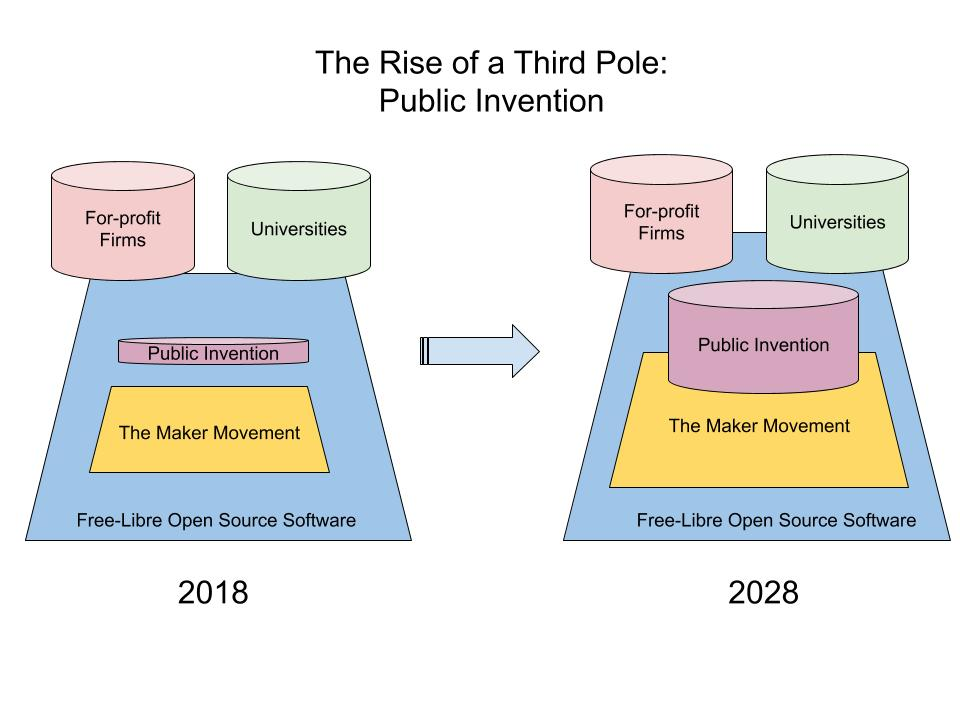
\includegraphics{figures/The_Rise_of_Public_Invention.jpg}
  \caption{The Rise of Public Invention as a Third Pole of Progress}
  \labfig{rise}
\end{figure}

With your kind permission, let me take you on an
imaginatvie journey into the near future of the next 20 years.

There will be three engines of economic growth:
for-profit research, universities, and public invention.
People will flow smoothly between these three poles.
A young researcher might start volunteering for public invention while
looking for a good job, move to that job, then go back to school
as a student or a lecturer,
then back to work, then back to public invention.
Profit is one of many tools of motivation, competing with
the status and recognition of universities and public invention.

When a person has a three-month hiatus between jobs or a
high school teacher has a summer off, it is easy for them to find
a public invention project to work on, because there is a
well-catalogued and maintained list of projects for them to match
their talents and desires to.
Everyone kind of knowledge worker can contribute, because
there is high demand for technical writers, photographers,
graphic artists, managers, quality assurance experts, and more.
Skilled makers can contribute PCB designs or hand-soldered boards.
Woodworkers, metalworkers, 3D print makers, and other craftspersons
can find a list of needs and quickly produce something contributing
to a project.

Universities remain exclusive, and people compete to get in as
both students and faculty.
Public Invention remains inclusive, and people compete to
be recognized for their contribution. Gratitude begins
to hold its own againt vanity.

The landscape of projects is driven by human curiosity and
altruism. Finding needs to be addressed by public invention
by adding to the list of potential projects is a recognized
contribution.

Everyone who wants a mentor can find a mentor if they are willing
to put their own time in to make the mentor's time well-used.

Material costs of projects, but not labor, is financed by
charities that serve an evaluative function on the projects,
guaranteeing donors that their gifts have high impact.

When a person has an invention idea, they have a choice.
They can attempt to monopolize it and have a small chance at
a large profit, or they can donate it public invention and
have certainty of a small recognition.

The current near-monopoly on sophisticated medical devices held by
large corporations has been eroded by open-source designs
created by public inventor in response to health crises that
began with the COVID-19 pandemic 20 years earlier.
A much greater competition by medium sized firms has led to
greater innovation. In the low and middle income countries,
medical care still lags the wealthiest countries, but is
clearly catching up rapidly.
Open access to medical data and training materials is a
part of this process. Colleges, universities, and clinics
have open-source versions of ventilators, imaging devices,
anesthesia machines, lowering the cost of training.

A growing public commons of free and open designs
across the entire spectrum of possible inventions
is mined by corporations and both large and small to provide
new devices at reduced research costs.

Universities have mostly abandoned patenting their research
and now by default release all of their work in open-access journals
and under open-source licenses. Universities compete with each
other not only the quantity and quality of their research, but
on their openness and humanitarian impact.

Philantrhopists and funding foundations provide perhaps three
dollars out of every hundred to public invention projects.

People go to parties and say things like ``I'm a public inventor''
and everyone knows what they mean.
Although just as today with open source projects, a majority
of public invention projects are never heard of, but
everyone once in a while someone will say in hushed tones,
``See that person with the ombre dyed hair? They were the
leader of the oxygen concentrator team in 2025.''

\section{The Far Future}

In 2112, the first class of Star Fleet Academy is matriculated.
Money is still in use for luxuries and to fund world wonders,
such as the first generation ship, but is irrelevant
for basic food, clothing, and shelter.

There are no 50 billion people on Earth and 5000 off-Earth
and inside the asteroid belt. The carbon footprint of human
society is now less than it was in 1945. Global warming
remains a problem but is the CO2 levels are declining.

Forms of art unthought of in 2022 are flourishing.
Most people know and care very little about public invention,
and are engaged in their own pursuits, but
the few who do live in a wonderland of possibilities.

Each public inventor has access to an enormous library of
scientific thought and access to design tools unimagined in 2022.
The average high school student can create designs of
complexity unimaginable in 2022, and can order them
produced at a reasonable cost.
Fabrication of integrated electromechanical devices is
done at the touch of a button.
The range of materials available for crafting includes
diamond, titanium alloys, fibers of unimaginable strength,
and intelligent polymorphic materials are approaching flubber.

Biohacking has reached new levels, driven by necessity and
pleasure. A student in England just made an English pea plant
whose pods open and spill out multi-colored peas like unzipping
a purse full of pearls.
There is tomatoes for 413 distinct micro-climates.
Luxury furniture is now grown in place as a single tree.

The Oceans are clean and productive. The by-catch has been
eliminated; only the fish that are actually eaten are taken.

The forests are half-way to recovering. People gather in forests
with the help of tree-climbing spider robots, which produce
food that was never worth gathering before.

The role of public invention in the success of the world is
debated. The Inevitablists claim that success was alway inevnitable.
The Constructivists claim that success was constucted based on
specific policy decisions, individuals, and organizations.

\chapter{The Stoic Point of View}

The ancient Stoics taught a practical philosophy that is only
tangentially related to the common meaning of the English word ``stoic''.
In terms of metaphysics, they believed that we should live in accordance with nature, and it is natural for humans
to use the reason gifted to them by the Gods, if they exist---the Stoics were not
Universally deistic or non-deistic.
The first principle of Stoicism is to
distinguish between that which you can control, and that
which is outside your control.
You can control only your own actions, and, with practice,
your thoughts. The thougts dye the soul.
You cannot control what others think of you.
The praise of others the clacking of tongues.
Being in the ``inner ring''---the faculty club,
or being invited to the exclusive conference, or
to Lady Boodle's dinner party, is not worth a fig.
\marginnote{
  I believe that in all men’s lives at certain periods, and in many
  men’s lives at all periods between infancy and extreme old age, one
  of the most dominant elements is the desire to be inside the local
  Ring and the terror of being left outside.
\url{https://www.lewissociety.org/innerring/}}
Alexander the great and his mule driver are both gone,
nobody remembers much about Alexander except his name.

The Stoics saw each of a part of a great community, each a
tiny part of a tiny society in a large Universe.
What is good for Society is good for the Individual.\marginnote{This is similar to the idea that we are all cells in the Body of Christ.}

Stocism is a great aid to the public inventor,
because it armors one against disaspoint and frustration.
It sees little value in accumulating enormous wealth.
It asserts that reason is a gift, perhaps a divine gift,
to be used for the betterment of all.
Even the spiders and bees have their useful occupation.
Some of us are born to farm, to entertain, to build, and
some of us are born to be public inventors.

The Stoics believed that reason was a gift to humans from the Logos.
The Logos might be interpreted as divine reason, or directly
as God or the Gods.
The ability to reason allows us to be more than beasts
and to participate, at least partially, in the divine.
That meant this in several senses.
Reason keeps us from being inebriated
all day, although as brutes we may find this pleasant.
Reason makes us behave civilly towards our
fellows, although it is, on the surface, to our advantage
to steal from them.
To them philosophy, literally the love of wisdom,
meant the study of how to live well.
Today, classes in philosophy are really the study
of the history of philosophy, rather than philosophy itself.
Because we are gifted beyond other animals in having
reason, it is our duty use our reason to learn how to live
well.
To the Stoics, this spanned personal hygiene,
to how to behave at dinner parties, to how to be a citizen
of your state, and even how to be a citizen of the world.

In the classical period of Stoicism, Universities had
not been invited, and their was no model for either
the private inventor or the public inventor of physical
inventors.
A small number of philosophers may have procured a
living by inventing the constructs of philosophy, but
even then only indirectly.
However, I assert that in the modern world, Stoics
should agree that being an inventor is a worthy profession
just like being a farmer, a policeman, or a teacher.

The Stoics cultivate {\em preferred indifference.}
They were not opposed to wealth.
It is better to be rich than to be poor,
but one can be good and happy while poor.
But they would agree with modern psychologial research
that once a basic level of material wealth is obtained,
additional wealth is not particularly valuable.
If you have enough, whether you have more than enough
or just enough should not make you unhappy in either case.
One may prefer to have more than enough, but one should
not be distraught at having less than enough.

Marcus Aurelius was strongly communitarian.
He wrote that what is good for the body politic (by which
he meant both the Roman empire and all humanity) is good
for the individual.
In general the Stoics did not have a strong sense of
an immortal soul.
They believed death was a transmuation of the elements,
and that is was natural for a person to be born, participate
in humanity, and then die.
The physical body was given by the mother, and
then by food, until eventually it was transformed back into
the elements from which it came.
The mind or soul came seemingly from nowhere and went
seemingly to nowhere; this should not be counted a loss
or a sadness, as nothing has been removed which was not
given as a temporary gift in the first place.
Humans, just like the plants, the beasts of the fields,
and even th insects, had their job to do.
In ancient Rome there was less freedom to choose
one's occupation than there is today.
To the Stoic, being good consisted in doing the assigned job
well, whether you were an ox, a slave, a soldier, or an emperor.

The public inventor uses reason on behalf of the
universal community without much regard for their own
profit.

It seems to me the Stocis would have approved of public invention.

\begin{itemize}
\item Basics of Stoicism
\item Nature and Reason
\item Stoic Communalism and Inclusivity
\item Stoic views on occupation (Aurelius, Epictetus)
\item Stoic assistance to the public Invention
\item Resisting the siren songs of praise, the ``in club''
  \item Resisting the siren song of excessive wealth
\end{itemize}


\chapter{The Christian Point of View}

\marginnote{I am a devout Unitarian. Most Christians would not call me a Christian,
  though I have been highly influenced by Christianity.}

We must admit from the outset that Jesus was not
an electrical engineer.
He never touched a soldering iron, though a soldier's iron touched Him.
There are limits to what the words attributed to Christ and his followers
can directly mean for public invention.

This is the Great Commandment:
\blockquote{
... and one of them, a lawyer, asked him a question to test
him. "Teacher, which commandment in the law is the greatest?" He said
to him, "'You shall love the Lord your God with all your heart, and
with all your soul, and with all your mind.' This is the greatest and
first commandment. And a second is like it: 'You shall love your
neighbor as yourself.' On these two commandments hang all the law and
the prophets."
}\marginnote{Matthew 22:35-40}

The great innovation of Jesus was Love.
The Stoics before Him and many other philosophies extolled ethics
and fine, civil behavior.
A Stoic would share their bread with you, out of duty.
A Christian would share their bread with you, out of both love and duty.
The love/duty duality is reflected in the great Christian debate
of the importance of faith (the Augustian view) and good works (the Pelegian view).
C.S. Lewis and most mature thinkers view them as intertwined.\marginnote{But not me---I belive good works matter far more than faith, a view which is officially heretical to many Christians.}

What is God if not the Creator, the Prime Mover, the First Maker?
Dare I say God is an Inventor?
To love God with all our heart, our soul, and especially
with all our mind, means to love and study His creation, creatures, and work.
I therefore consider all sciences, not least mathematics, to be branches of theology.

The second part of the Great Commandment is to love you neighbor
as yourself.
Surely this means that I must share my inventions and knowledge
with my neighbor just as I share my bread.
The Great Commandment requires sharing, and sharing requires
free-libre open source licenses.
Free software and free hardware is therefore a Christian commandment.
Some us are surely
meant to be public inventors and to love our neighbors
by providing them open-source ventilators and machines to provide clean drinking water.

The parable of the talents (Matthew 25:14–30)
may apply. A ``talent'' was gallon jar of silver coins, but
the parable was metaphoric to begin with, and we can
by happy coincidence use the normal meaning of the English word
``talent'' here.
Talents must not be buried!
Surely those who have the inclination to study math and physics
have a talent, because assuredly not everyone is so inclined.
There is support for this idea from St. Paul as well:
\blockquote{
  Whatever your hand finds to do, do with all your heart.}
(Ecclesiastes 9:10)

In Ephesians, Paul establishes the metaphor of the ``body of Christ'',
which parallels the Stoic view of the community of humanity.
\blockquote{
  11 So Christ himself gave the apostles, the prophets, the evangelists, the pastors and teachers,
  12 to equip his people for works of service, so that the body of Christ may be built up
  13 until we all reach unity in the faith and in the knowledge of the Son of God and become mature, attaining to the whole measure of the fullness of Christ.

  14 Then we will no longer be infants, tossed back and forth by the waves, and blown here and there by every wind of teaching and by the cunning and craftiness of people in their deceitful scheming.
  15 Instead, speaking the truth in love, we will grow to become in every respect the mature body of him who is the head, that is, Christ.
  16 From him the whole body, joined and held together by every supporting ligament, grows and builds itself up in love, as each part does its work.
}
(Ephesians 4:11-16)

This same idea, that each of us has a precious originality,
has the modern catchphrase: Don't forget to be awesome.
``Awesome'' in this case means to be your true self.
I personally believe this is the meaning of ``salt of the earth'' saying:
\blockquote{
  13 “You are the salt of the earth. But if the salt loses its saltiness, how can it be made salty again? It is no longer good for anything, except to be thrown out and trampled underfoot.
}(Matthew 5:13)
This idea is echoed by C.S. Lewis:
\blockquote{
  “Even in literature and art, no man who bothers about originality will ever be original: whereas if you simply try to tell the truth (without caring twopence how often it has been told before) you will, nine times out of ten, become original without ever having noticed it.”
}(Mere Christianity)
The Public Inventor must choose projects as the inner light guides them.
The choice of what to work on cannot be reduced to an algorithm.
The work of invention should be a thrilling, joyous adventure.
There will be drudgery but the work itself must remain loved
by the inventor.

Jesus was many things, but by tradiditon his profession
before his ministry began is translated into English as ``carpenter'', but
David Bentley Hart has more recently translated the Greek ``tectos'' as
``builder''\cite{hart2017new}. Jesus was a builder. It is not a play on words to say
He was a Maker.
According to the gospel of John and the Athanasian Creed which enshrines
the Trinity, Jesus was the Word\marginnote{The Greek in John uses ``Logos''. The logos is of exceptional importance to the Stoics, where it can be translated as
  ``reason'' or ``nature'' or ``divine reason''.}and the Word with God at the beginning,
so was also the Maker.

Christians are called to be ``Christ-like''. This is not usually interpreted to mean,
``be a maker if you are given a God-inclination to make'', but I see this as
a Biblically supported view.
C. S. Lewis would have us be ``little Christs'' and ``put on Christ''
by trying to be like Him, without imagining that we really are like Him.
I don't think Lewis meant to apply this directly to a person's vocation.
Nonetheless should not an inventor attempt to make holy inventions to the
extent they can?
As I have said before, all inventions can be misued and corrupted, and
I suppose atom bombs may someday be good for something.
But if anything is ``unholy'', neutron bombs,
poison gas, and land mines are.
Vaccines and solar panels are close to the ``holy'' side of the ethical spectrum.
Therefore the Christian inventor is called to consider the impact of
their inventions beyond the narrow confines of their paycheck,
and to make humanitarian inventions.


The great challenge facing us at this writing is
global warming.
The primarily requires policy changes; we cannot
invent our wait out of this problem, because the
use of inventions is always optional, and some people
just want to watch the world burn.\marginnote{
  Alfred Pennyworth : Well, because he thought it was good
  sport. Because some men aren't looking for anything logical, like
  money. They can't be bought, bullied, reasoned, or negotiated
  with. Some men just want to watch the world burn. --- The Dark
  Knight, 2008
}
Nonetheless, academics and for-profit firms have
already given us inexpensive solar and wind power and electric cars.
I hope that public inventors contribute as much in the next twenty years.

\section{Stewardship}

Do I have anything new to add here?

\chapter{Universal Salvation}

Possibly the world will become more inequitable over time,
although I do not belive it will; that would not be much fun.
Whether it does or not, we can expect the current trend
of poverty reduction to continue. At the time of this
writing there are many readers who will scoff at the
idea that poverty has generally been reduced over time
and the last 40 years in particular, though I suspect most
of them are not old enough to remember the 70s.

Ideas have a life of their own.
This is a figurative statement, but it might be literally
true as well.
The Public Inventor must act as an agent for good, but
each of us is called by some ideas more than others.\marginnote{I am fascinated by tensegrities, for example.}
It is no good treating invention as a drudgery; it should be a joy.
The Public Inventor will be most effective when working on an invention that calls to them,
whether they originated the project or not.
Therefore many public inventions will not directly make the world more equitable.
Almost every invention helps someone more than others; this is to be
expected.
Nonetheless, when all else is equal we should work on inventions which
make the world more equitable, rather than less equitable.
Certainly, the enormouse space of inventions which decrease povery
and decrease inequity is a rich and varied playground which
none will exhaust.


\begin{itemize}
\item Small is Beautiful
\item The road to the stars runs through villages and slums
\item None of us are free until all of us are free
\item Anthropomorphised money does not love poor people
\item Nor does it love rich people.
\item It wants to accumulate.
\item But people love people--we can motivate volunteers this way
\item We cannot live together on spaceship earth while we have grinding poverty
\item Cutting your own carbon footprint in isolation is of limited value compared to political action---yet we are “sold” such ideas.
\end{itemize}


\chapter{Social Inventions}

Advances in ``hard'' inventions
have made public invention easier,
but ``soft'' inventions also play a role.
In particular, practices pioneered by the Free Software movement,
such as the way projects can self-organize and use
free software and hardware licenses, enable running a
project and sharing it freely.

The free and open-source software has developed a set of cultural
practices that allow teams to work together.  These include:
\begin{itemize}
\item cultural dissuassion of unnecssary splitting or ``forking'' of a
  project,
\item using recognition as an incentive for contributions,
\item using version control systems to manage contribtuions,
\item and using Agile software methods and big visible charts to
  manager work.
\end{itemize}
\marginnote{``The Apache
  Way''\url{https://www.apache.org/theapacheway/} is a valuable
  starting point, as is ``Homesteading the
  Noosphere''\url{http://catb.org/~esr/writings/homesteading/homesteading/}
  and my own work, ``How to be a Programmer''
  \url{https://github.com/braydie/HowToBeAProgrammer}}

An additional practice is that documenters and maintainers
are valued nearly as highly as software coders\marginnote{Eric S. Raymond has explained this in his essay ``How to Become a Hacker'' in in the ``Status in the Hacker Culture''
section\url{http://www.catb.org/~esr/faqs/hacker-howto.html}\cite{Raymond1999}} here.
This is a cultural practice which is of paramount importance
to public invention as a movement.
Often, an invention has a kernel of math or ingenuity
that can only be created by someone well-versed in the
appropriate science and art.
However, public invention is a team sport.
Every contribution must be honored and valued.
In some sports, some positions naturally have more
opportunities for drama---the striker on a football team,
the pitcher on a baseball team.
But teamwork is essential to winning.
Those who manage projects, write documentation,
help with quality assurance and provide financing are
equally important.

The value of these cultural inventions cannot be overestimated.
But the creation of the GNU General Public License (GPL)
\marginnote{The work of the Richard Stallman and the Free Software Foundation in the creation of the GPL has inspired many other licenses
  practically created the field and practice now called ``free culture''. This goes far beyond the GPL, but we can use the GPL as the
  originating event for these other licenses.}
is of equal importance.
The GPL is brilliant in its simplicity: it gives the
user the right to modify and distribute a copyrighted work
and works derived from that a copyright work so long as
the distributor does not attempt to monopolize the works
and gives the derived work freely under the same terms.
The GPL and related Creative Commons licenses give
creators control over how their work is used.
In particular, they may choose to enable re-use, which
is the point of public invention.

There are also reciprocal licenses for hardware.
Hardware designs are not covered by copyright, and
so they are fundamentally different.
However, this is of no concern to the public inventor,
who as a matter a principle is giving away the invention
for the whole world to use freely.
It would be nice of those who take a device and made
improvements to it would contribute those improvements
back to the project and the world as the GPL forces
in software, but at present our legal structure for
doing this is weak.
We may, however, rely on the ``honor system'', which
can be astoundingly effective in practice.


\begin{itemize}
\item Practices pioneered by the Free Software Movement
\item Internet community
\item Open Source Software paved the way with certain teachings
\item Projects need leaders
\item Projects run on the coin of acknowledgement
\item Maintainers and documenters are highly valued
\item Licensing matters, but has been pioneered
\end{itemize}

\chapter{Building a Public Invention Commons}
\begin{itemize}
\item The value of a Commons
\item The value of Commons of Problems
\item The value of a Commons of Solutions
\item Don’t worry, be crappy.
\end{itemize}

\chapter{Limits}

Love matters more than lasers.

All inventions can be repurposed to ill.

Public invention is likely to spawn many for-profit firms that will make millions,
but public inventions do not confer monopolies.
It will be difficult for firms to make billions from public inventions.

You can make yourself lovable but you cannot make someone love you.
No matter the good that public invention accomplishes, haters gonna hate.

We cannot invent our way out of ignorance or hatred.

\pagelayout{wide} % No margins
\addpart{How to Be a Public Inventor}
\pagelayout{margin} % Restore margins

\chapter{How to be a Public Inventor}

\marginnote{ The chances of your success are zero, but the importance is infinite; therefore, I support you. -- Sir W. Lawrence Bragg}

\begin{itemize}
\item Motivate yourself through love of humanity, life, and knowledge
\item Publish early and often
\item Don’t seek patents
\item Publish your failures
\item Seek community
\item Help other Public Inventors
\item Ask for Help
\item Learn by doing
\item Failure in service to a big idea plants the seeds of success.
\end{itemize}

\chapter{Money and Volunteerism}

\begin{itemize}
\item Despite appearances, more of us have more time than ever before
  \item Gandalf ``All we have to do is to decide what to do with our time.''
  \end{itemize}

\chapter{The Emotional Intelligence of the Public Inventor}

Invention means creating something that has never been
created before.
By definition, the Public Inventor is doing something
difficult.
True creation is a both a satisfying
joy and one of the frustrating slog.
By articulating some of the emotional difficulties
they will likely face, we hope to prepare them.

\section{Getting to the Coal Face}

The first problem faced, even before any insecurities,
is ``getting to the coal face.''
This means specifically learning enough but a particular
area to have some discernment on what constitutes a good and new idea.\marginnote{This expression can also mean ``doing the nitty-gritty'', I do not mean it in that sense.}
When I was a boy, I tried to think of a perpetual motion machine.
I excuse myself because of my age; but only just.
Although I didn't know it at the time, I had no right to be
thinking about that problem because my entire knowledge of
thermodynamics was the use of the word ``entropy'' in a Fantastic Four comic book.
I was not at the coal face---I had not done the work, analogous to traipsing
deep down into the mine to where the freshly exposed ore was---and so could
hope to do no real work.
A person who does not get to the coal face is either ignorant,
as I was, or a quack, as I hope not to be.
We must treat the ignorant gently, becuase often it is not
easy to tell if you are ignorant or not.

One of the easiest ways to tell if some one is a quack is
to see if the have gotten to the coal face.
That is, can they intelligently discuss the details
of particular specialized area pertinent to their invention?
If they cannot, their attitude will determine their fate:
the merely ignorant will take the discovery that they
do not know as a signal to study further, even if dejected by it.
The quack will attempt to deny reality and become combative.

For the sake of the young especially, we must never say
``No, you are wrong'' without also saying ``but it was
a good try, and if you study this and that, something may come of it.''


\section{The Insecurity of New Ideas}

For example, I recently discovered something of
real if minor scientific value---or so it seemed to me \url{https://github.com/PubInv/segmented-helixes/blob/master/doc/StackingHelix.pdf}.
This is quite unusual, and the more valuable something is,
the less likely it is that we are the first to think of it
or develop it.
Extraordinary claims require extraordinary evidence (ECREE),
the so-called Sagan Standard \url{https://en.wikipedia.org/wiki/Sagan_standard},
is fundamental to all scientific emprise.
I of course did about ten hours of searching to
attempt to verify that it had not appeared in writing before.
However, even after working on it for six months and preparing
the publication, I was riddled with doubt that this might simply
be so well-known that nobody bothered to write it up.
In an attempt to allay my fears, I asked for help, and
I think an anonymous person said it was not valuable and ``pretty simple''.
Nonetheless, reputable journals continued to publish work
which completely subsumed by my work. COVID-19 delayed the
in-person conference where where the work was accepted.
I remain in a state of emotional trepidation about this work,
and unable to judge if it is quite signifianct or trivial.
Many public inventors are going to be in precisely the
same position.

We will be most effective if we can put aside our egos
without decreasing our emotional involvement in the work.
I care about the outcome of this research, in part because
I simply love mathematics itself.
I am not ashamed to say I love my work. If it turns out
to be insignificant or previously published I will be disappointed.
However, we must not allow such sentiments to cause
us to be in anyway biased or discouraged.
We must at all times hold forth the highest standards
of honesty and academic integrity.
It is our duty to publish results; in a sense,
this is therefore self-promotion.
But we must not over-sell or exaggerate our accomplishments.

\section{The Dreaded Scoop}

About twenty times in my career as a Computer Scientist and Public
Inventor I have somehow informally presented an idea to someone or a
group of people, only to hear them say, “That’s been done.”  Sometimes
they add some additional information about who and when, but often
their memory is vague.  To a would-be maker, inventor, or researcher,
“That’s been done” can feel like a punch to the solar plexus.

My advice is: Don’t you believe it.

All of the twenty times I got that sinking free-fall feeling in
response to “thatsbeendoneism”, and I took notes and researched what I
was told. Approximately once it turned out to really be true.  The
other 95\% of the time, the work mentioned in no way decreased the
value of the project I was undertaking, and even validated
it. Sometimes it seemed to have no relation whatsoever. Sometimes it
was tangentially related, but the previous researchers had taken a
very different approach. Sometimes they had begun and stopped, and in
the twenty intervening years the march of technology, and even
mathematical theorems, has since opened up new vistas.

I don’t like the way the word “privileged” has come to be used in the
last 20 years, but in that usage of the word, as a researcher, I have
been. I can be an over-confident ass, with the redeeming feature of
complete blindness to my own ignorance. I am anti-fragile. Yet, I
suffer from the impostor syndrome and insecurity, just like everyone
else reading this, I suppose.

Judging by the emotions I personally go through when I hear “That’s
been done”, I’m sure those words have prematurely killed many a fine
and interesting research project, invention, or even DIY craft
project.  We must forgive the thatsbeendoners, and understand
them. They are genuinely trying to inform us. However, the human
weakness of a desire to appear knowledgeable combines with the human
frailty of not listening patiently enough to our ideas before passing
judgment, multiplied by the human limitation of memory. The result is
that most of the time when someone says “That’s been done” you should
carefully note what they say, plan to carefully research it tomorrow,
and not worry too much.

Many research topics can go in about ten different directions. Any one
researcher may have considered two of them; the other eight are open
to you. When this is not true, you will likely know, because these
become recognized under the moniker “open problems”.

Do your homework and spend a lot of time in the library or researching
online. When you have done that, work boldly and confidently in
whatever direction your spirit guides you.

\section{Publication}

By definition, the public inventor publishes.
This can take many forms, but the most challenging and most rewarding
is academic peer-reviewed publication.
Society has creating a beautiful machine, which we might
call ``the body of human knowldege'', or, more colorfully, the exobrain.\marginnote{Tony Stark, eat your heart out!}
The internet and the trend toward open-access publishing has made this
knowledge more accessible at lower cost and more widely shared
than ever before.
Google deserves a hat tip for their role in this, which has made
``to google'' an understandable verb.

Long before their was the internet, it was systematically categorized
and edited. In fact, we can think of the peer-review by qualified as
reviewers as the best editorial function in terms of selecting what
is worthy.
Nothing stops you from publishing your work on the internet, but
without peer review your potential readers must make a higher investment
finding, evaluating and validating your work for themselves.
In a sense, a paper worth 10 microfullers by itself is worth
20 microfullers when placed in a journal because of this
editorial and validating function.

Academic publication lasts approximately forever.
The exobrain is an gift that keeps on giving.
If you could receive some sort of money or karmic value
for your work, academic publication is the best way
because it would keep paying you year after year as
your work assists others. Sadly, this is not possible
today, and the only people who derive economic benefit
from academic publishing are the harried and beleagured class of assistant professors.
In fact, because today you often have to pay open access fees, academic
publishing is a slight economic detriment to the author.
But it is a tremendous unrealizable economic benefit to your
sibling scientists.

Publishing is, however, tedious for the public inventor.
The quality bar for preparation is quite high.\marginnote{The decrease in the cost of paper
  publishing the low-end of the spectrum of publishable quality has been expanded, which I consider
  a good thing.}
Finding an appropriate venue for publishing takes about half a day, and
then there is a high margin for error, even after reading papers in many
different venues.\marginnote{Professional academicians don't have this problem, but we cannot expect
  everyone to stay on top of all journals and conferences in a field.}
Finally, it takes months to receive a reply and often it appears
the reviewers spent about twenty minutes reading the work and didn't seem
to really understand it.
Then, you may get rejected, and when you are not rejected, you often
have additional work, sometimes substantive but usually just formatting to do.

Despite these troubles, I strongly encourage inventors to pursue
academic publication for those works that deserve it. At Public Invention
most of our project aim for a acdemic publication from the first day,
but other projects are art projects or exploratory in natue.
Having a posse---siblinghood of technical friends who can advise you---facilitates this decision.

\section{Humility: Be Foolish}

An invention project which is guaranteed of success is hardly worth the name.
The public inventor must therefore be prepared to fail.
Sometimes we learn the universe is harder to manage than we thought;
this learning is valuable.
Sometimes we learn that we have been foolish.
This is an equally valuable lesson, though it can be a jagged little pill
to swallow.

\section{The Glory and the Impossibility of Comprehension}

The Universe is ``Infinite in All Dimensions.''\cite{Dyson1989}.\marginnote{“Space is big. ... I mean, you may think it's a long way down the road to the chemist's, but that's just peanuts to space.”  -- Douglas Adams, The Hitchhiker's Guide to the Galaxy}
When Freeman Dyson titled his book of essays that, he did not mean
only in the spatial dimensions.
It appears to be infinite as we look out and as we look in.
It appears to be infinite as we look at the large and at the small.
Human progress has created, or perhaps has been driven by,
an ever expanding understanding of the richness of the creation
we inhabit. Most recently, the discovery of thousands of known
exoplanets implying a galaxy full of them, is a spectacular example.

There does not appear to be any end to new art forms, and the
old art forms are made large by the creation of the new art forms.
Photography has not hurt painting.
Recorded music has not hurt music in general.\marginnote{It has decreased the breadth of musical mastery in the general population.}
Free verse\marginnote{\url{https://quoteinvestigator.com/2021/05/24/poem-tennis/}During the question period afterward, someone asked: “Mr. Frost, do you ever write free verse?” and Frost gave his famous answer: ``I would no more think of writing free verse than of playing tennis without a net.''
Vance spoke to the U.S. poet Carl Sandburg and presented his rejoinder:
`` ... I would have him know that I have not only played tennis without a net but have used the stars for tennis balls.''}has not hurt poetry.

Amongst this embarassment of riches the public inventor
may feel a little small.
You can study all day for years and not master a single corner
of the sciences, and most of us cannot make that investment in
first place.
I personally feel that I cannot master even differential equations
and basic electronic circuits.

However, we must support each other in our attempt to learn what we can
in our brief time here together. It is not a question of knowing everything
about anyting, but a question of what we should invest in learning.
In this, the inventor has an advantage over the specialist:
invention is often the combination of elements from disparate fields.
The public inventor gets a pass on studying anyone one field,
in exchange for a demand of voracious study of many fields.
I personally could live no other way.\marginnote{It is a personal shame of mine that I know almost nothing about chemistry.}

\section{Feeling Unappreciated and Ignored}

Somtimes the fruit of your labor sinks without a trace.
Time and time again, great work has been ignored, only to be
rediscovered, with great praise and thanks, thirty years later or more,
when the original author is dead or has been denied tenure!
And those are the lucky ones.

Sometimes an idea is ahead of its time.
However, it is also entirely possible to do excellent work, and simply
receive blank stares and yawns and in fact the work may never
mean anything to anybody.
This happens to artists fairly commonly.
The only remedy when this happens is to do some other excellent work.

Working hard on a project for a long time that is completely ignored
almost always positions you better to do some other project.
I suppose it must happen that this is not always true,
but it has never happend to me.

\section{Patent Envy}

There is a mystique around patents.
The word ``patent'' is sometimes pronounced with certain
breathless excitement, as if it confers success, riches,
or some proof of merit.
Don't be fooled---it gives none of these things,
and costs money and time.
About the best thing I can say about the patent system
is that provides an extremely well-organized and useful
database of clearly explained ideas.
This is still used for, but was more useful
when paper publication was the only route.
However, it should have no mystique.
By making an invention sufficiently narrow, it
is possible to get a patent in almost any field.
This does not mean it has any value to anyone.


A patent provides a monopoly for 20 years on some idea.
This is antithetical to the entire premise of public invention.\marginnote{All of humanity is in peril of extinction if each one of us does not dare, now and henceforth, always to tell only the truth, and all the truth, and to do so promptly — right now. --- Buckminster Fuller.}
It made more sense when publishing ideas was harder.
The long monopoly did not seem so long when the patent system
was established in 1790.

Patents do occasionally prevent large firms from using the
work of individual inventors without compensation, which
is a positive feature. However, more often they are collected
by large firms who finance their issuance from flimsy actual
innovations and then use them to compete with other large firms
and to create barriers to entry to the market for small firms.
It is an idea that was useful in its time and in its form,
that utility is now passed, and the patent systems needs
to be reformed.

There are people who will passionately argue that without
the monopoly provided by patents nobody would research new
drugs, for example, or other useful inventions.
There has been plenty of great research in software and
mathematics which luckily was only slighlty tainted by patents.
Being the first mover in a market with an invention provides
a tremendous financial incentive.
If those prove insufficient, society could finance
pharmaceutical research through taxation or
even donations.
However, public policy should not influence
what the public inventor does.

The question is: will an invention serve the public better
by being patented? The answer is usually no.

Patents give the inventor the right to file for one year
after a public disclosure. Furthermore, by law,
all inventors must be named in the patent. Both
of these stipulatons are nearly impossible to accomplish
in the modern, open-source way of working.
The modern way to develop is to work ``in the light'',
not keeping one's work secret.
Since public invention invites broad participation on projects,
there are often dozens of volunteers that work on a project,
and sorting out who contributed what is a thorny nightmare.

Whatever one may think about patents, they have no
place in public invention as a movement.

\section{The Need for and Difficulty of Fellowshp}

There is no more secure entry to friendship than a shared passion.
The public inventor often wants friends, and wants to share
their passion.\marginnote{A detractor could argue I am writing this book to have a lot of virtual friends.}
Often, even when working in the light, this need
is hard to satisfy.

In an all-volunteer project in which nobody gets paid,
volunteers are ephemeral. They may come and go.
Sometimes they are seeking to learn but are not
really ready to contribute, and cannot really
be a peer.
In some circumstances, people are simply jerks.

\section{Mentorship through Collaboration}

Public Invention’s motto is “Invent in the public, for the Public.” Inventing in the public means working “in the light”---letting everyone see the work product as you go along. In a sense, working in the light is a form of mentoring that is available to all for free.

But people need one-on-one, personal mentoring as well. I learned so much from my personal mentors and other influential people in my life (some of whom probably wouldn’t remember me) that I personally feel it is a universal duty for each of us to mentor whenever we can. Here is what I try to do.

The best mentorship is collaboration. The most lasting insights I ever got were from watching my father solve a computer programming problem. He offered no advice; he just solved the problem out loud with me looking on. In fact, he reconstructed Bresenham’s line drawing algorithm, I’m pretty sure without ever having seen it, from first principles, writing neatly on a sheet of graph paper. We programmed it in assembly language on my TRS-80. It could draw lines across the screen so fast you couldn’t see them move. In 1979 on that computer, that was a big deal.

My second mentor, Dr. Martin L. Smith, worked closely with me on certain problems in geophysics and then closely guided my reverse engineering of Hypercard for the Sun Windowing system in 1987. This was better than any mottos he could have produced. We wrote a paper together, and in that way he demystified academic publishing for me.

I had the pleasure of coding for an hour with Kent Beck. It was a very informative hour, even though we did nothing that he hadn’t already written about in a book that I had already read.

I try to work directly with people as colleagues whenever possible. Sometimes this can be done in near equality; for example, a recent volunteer, Lauria Clarke, was a better PCB designer than I was, and on that project we could be equals. In other cases, particularly when it involves pure computer programming, I am so far ahead of a student that there is no point in pretending we are equals. In these cases the teaching is asymmetric, but it is still focused around collaboration: we are getting something done together, and if I may be doing most of the typing and coding, we are still doing it together.

Occasionally young people appeal to me for career advice in various ways. I am of course honored by this, but approach it with great humility. I have only lived one life and I’m not at all sure that I’ve done it successfully, so I can’t tell anyone what to do. But I can share a lot of experience that may be relevant. The mentor must always be humble.

Young people are inexperienced. They may miss major opportunities because they simply know nothing about a possibility. You may greatly help young people by sharing such experiences, and allowing them to take what they can from it. For example, I went to college, failed disastrously to be a physics major, and then succeeded in computer science. I went to graduate school and had some dismal experiences, though I eventually graduated, and am glad I did. I share failures and successes in equal proportion, because for most of us, that is what life is.

I try to be upfront about my biases. For example, if someone is trying to decide if they should go to college or graduate school, I tell them before we start talking that I will likely always say “yes, you should.” With that out of the way I try to listen with an open mind.

My face doesn’t show it, but I am a deeply enthusiastic person. This level of intense enthusiasm and optimism can, I’m sure, be off-putting at times. It is sometimes nice to have someone telling you that you can do anything, that no endeavor is beyond your reach. That is what my heart says. It is not always true.

But it is true that trying and failing is almost always better than not trying. I know this from experience; it is a percept, not a concept. Efforts often fail to produce their goals, but they rarely fail to produce some unlooked for result that falls into your lap like magic. Perhaps my greatest mentor of all, my grandfather, taught me a little homespun wisdom. Like all wisdom it is simple on the surface, but surprisingly deep. “You can’t catch a fish if your hook ain’t wet.” It means taking an action is more important than talking about the action. You can’t win if you don’t play.

In the end, I can do neither more nor less than share the light that has been shared with me.


\section{The Darkside: Going Closed Source}

During the great pandemic ventilator rush of 2020,
there were several teams that made high-quality
open-source ventilators and respiration tools and
then chose to continue developement in a closed manner,
probably because they enterred contracts with manufacturers
who either pressured them to do so or took over development
and were unwilling to continue in an open source manner.

I personally suspect many of these contracts ended
up being ``catch and kill'' operations; that is,
the teams got only a piece of future profits, and
the firm had no incentive to make the devices.
Thus the ``killed'' the project, and removed a potential
competitor, and nobody was helped at all.
This may have occured unintentionally.

Because the open source licensed for hardware are
more delicate than the GPL for software, going
closed-source in these cases may not have violated
the law, but certainly violated the spirit of the
projects when they said they were open-source.
It also violated the expectations of most
of the people (myself being one of them)
who supported those projects with money,
equipment, and time.

To bring inventions into practice, we need
for-profit firms. The natural life-cycle
of a public invention is to mature into
something that can make a lot of money
for someone who takes on the effort and
risk of manufacturing and distributing it.
Profit is good; monopoly is bad.
It is essential to public invention that
enormous amounts of money be made from public inventions,
and in general only a small fraction of that money,
if any at all, will go do the inventors.
However, the key is to keep the invention
free and open so that it may be improved
and constructed by anyone, including firms
which are competing with each other.

If a firm comes to you and says
``We will make this invention, but only
if you make the project close-source so
that we may have a monopoly'', you should
say, ``No, that is not in the spirit of public invention.
However, you are welcome to exercise the rights
already given you by the licenses we have used to
publish our work.''

A copylefted work may be continued as a
close-source work only by the copyright holders.
Since a public invention team may be diverse,
this may be problematic. However, if all copyright
holders agree to continue the work in a closed-source
manner, they may do so and the previously published
work remains a free and open project.
However, the world will benefit more if the
work continue ``in the light'', and that
is more in the spirit of public invention.

When a work goes closed-source, it tends
to become invisible.\marginnote{``Very hard to see, the dark side is.''}
This deprives the community of not
only the work itself, but even knowledge of if the work is
progressing.

\begin{itemize}
\item Getting to the Coal Face X
\item What to do when you are scooped X
\item Dealing with publication X
  \begin{itemize}
\item Rejection
\item Timeliness
\end{itemize}
\item Surviving being foolish X
\item Investing in learning without pedantry X
\item Feeling unappreciated and ignored X
\item Fuller’s theory of technological maturity and ripeness
\item The need for friendship and siblinghood
\item The siren-song of closed intellectual property
\item Patent envy and the patent mystique X
\item Dealing with disappointing teammates X
\item The insecurity of insignificance
\item Competition is obsolete
\item St. Exupery’s comfort of mediocrity - 20 bad sculptors are needed
\item “A walk-on part in a war or a lead role in a cage”
\item Paul’s call for each to do their part: Ephesians 4:11-16
\item Small is beautiful
  \begin{itemize}
\item Giants are built from small accomplishments, as long as they are published.
\item Thinking small is often a useful constraint.
\item Nothing does big things as well as doing small things.
\end{itemize}
\end{itemize}

\section{Anti-quackery}
\begin{itemize}
\item Litmus tests
\item Do you understand why Free Energy is nonsense?
\item Do you understand basic thermodynamics?
\item Do you understand Conservation Laws:
\item Mass
\item Energy
\item Momentum
\end{itemize}


\chapter{A Publishing Disconnect between the Free Software Movement and Open Science}
\label{chap:publishdisconnect}

\section{The Problem is Terminology}
Academic researchers and the Free Software Movement (FSM) use the word publish differently.
The difference in meaning in the word publish (and publication) creates a disconnect when the Free Software and Academic communities try to collaborate or when Academy adopts the ethos inspired by the Free Movement and the Creative Commons community, as we learned at a recent hackathon on behalf of Project Drawdown.
Publication:
Free Software Publication means putting anything, no matter how trivial or unrefined, online and potentially accessible to world, expecting it to be revised periodically and possibly linked to by others.
Academic Publication means putting a work in academic journal after it has been critically reviewed and circulated for review by peers and trusted advisors, where it will be eternally unchanged, and possibly referenced by others.
Free Software culture expects that works are “published = made accessible and known to a limited audience” from day one. Academic researchers often expect that things are not “published = announced in a peer-reviewed forum” until they have been thoroughly vetted and refined. This difference in expectations can challenge free software developers and academics who work together on projects. Nonetheless, such collaboration is extraordinarily useful and becomes more so every day. Creating a productive working relationship means creating a common understanding about expectations, the language used to describe the process, and the process of implementing the project.
This essay is an attempt to explain this to facilitate these communities working together.

\section{The Mutability of Published Works and Expected Quality}

Expectations in the FSM are that works are eternally mutable: they are constantly improved and are never in a final state. In a free software project, the contributors may not know who will make the next improvement, since in theory a wide audience is invited to contribute. Contributors are recognized rather discreetly, sometimes not even by name, in the commit logs and spread out in comments throughout the code. Contributors to a free software project are not individually responsible for its overall quality.
In academia the expectation is that a definite list of authors will take responsibility and great care for moving the work from conception to final, published state, after which it should not need any serious revision. Academia demands non-repudiation: each author is expected to stand behind the conclusions of the work with their reputation.
Free software is “published” immediately. By published, free software authors mean it is available for anyone who cares to discover, to examine, comment upon, and and even build a rival to. There is no expectation that the work is highly usable, let alone finalized. Everyone accepts that some bugs will exist. In fact, the expectation is that you will make it available before having a confidence it is bug free! Functionality often is achieved before all of the possible ideas the original author have come to fruition. The ethos of “release early and release often” embeds this idea. Well after first publication a project will reach the first point of functionality. At that point free software authors will frequently make a “release.” The “release” of an open source software project is symbolic; it is an assertion of readiness rather than a revelation of information. Once a “final” release has been published it is a indication that the authors believe it has some degree of usability. To working programmers, the release is a non-event; the development process immediately continues to revise the code base to add more functionality and fix any bugs, which are expected to be discovered in the previous release.
\section{Quality Standards}

Academic publication (and traditional writing at large) has a
different standard to meet for publication, which is a momentous
event. The work product is the explanation of an idea. Authors are
judged and criticized on how accurate or complete the idea
is. Significant flaws in the idea or its explanation are problems
indicating that publication and sharing the idea was
premature. Publication is a seal indicating a level of quality and
finality. Not only does free software not have this sense of finality
but the standard for quality, minimal functionality, is entirely
different. Typically in academic publication there is no similar
standard to being functional. English prose can only express an idea;
to the extent it is a “useful” idea (as opposed to just an abstract
idea) it requires someone to apply it through more work. Free software
has the advantage of doing work in its current state, typically
without the user even understanding the ideas expressed.

Free software developers often expect works to be accessible to anyone
or “Open from day one”, even before anything useful is done. To them
published does not mean publicized. The expected audience of a nascent
project is tiny. Nonetheless, developers expect the underlying ideas,
goals and data involved to also be shared publicly. They will expect
every mistake and half-way step will be made freely available to any
party that cares to go looking. They will not be concerned that
mistakes will reflect poorly on them early in the process and expect
to be judged on the progress and the process initially and only on the
quality of work when the developer specifically states they believe it
is high quality. Software is never “done”.

In contrast academics have the expectation that works are only shared
broadly with others when they have reached a final “done” or permanent
state. The final, permanent state requires that the first publication
be of high, even meticulous, quality and free of all serious
flaws. The finality of the state turns the work into an artifact that
allows others to judge and critique it as soon as it is published. Any
reputational impact rests on the state of the work at the moment of
first publication. Academic publishers seek to be respectful of their
readers’ time by producing the highest-quality work possible.

Free software developers have the advantage of being able to layer the
fixes over there bugs that get buried in the revision control
history. Academics mistakes are hard to correct silently once an
article has been published.

\section{Rivalry}

In some cases there is a race to reach this final point of publication
since reputational interests are disproportionately granted to those
who publish first. Those who follow cite previous works, increasing
the reputation of the previous works. In academia, sharing too much
too soon might enable someone else to craft a publication that
preempts the work and the reputational rewards that it
carries. Authors of an academic paper circulate select drafts of the
paper before publication to only a few individuals the author
trusts. The author hopes that any criticism will be in private and
that the carefully selected reader won’t attempt to compete or usurp
the opportunity to be the first to publish by rushing to the presses.

FSM developers expect that anyone could look at the work in progress
and criticize, contribute to, or be inspired to create a rival to, the
work. These activities have largely been embraced by the free software
community and turned into opportunities to accelerate the progress of
the body of free software generally. Rival works are common and to
some extent validate the value of the work they seek to supplant. It
is impossible to count the number of competing GNU/Linux
distributions, LLVM has long been competing to supplant GCC as the
default compiler in the free software world. These rivals encourage
diverse approaches until one dominant modality emerges, which can only
rest on its laurels for so long. As an example, in the important field
of version control systems, RCS was replaced by CVS, which was largely
supplanted by SVN, which lost to a competitive field of distributed
source code control systems, until git as emerged as the dominant
player.

\section{Method of Reuse}

Despite the different understandings around the meaning of “publish”
and the expectations that come with the act of publishing, there are
many similarities between writing an academic paper and developing
free software. Both recognize the need to build on the works of
others. Academic papers do this through a rigorous method of
citation. Free Software does this by incorporating libraries written
by previous authors into the work, or by modifying existing software
directly. Both methods of production also recognize the need to
circulate works prior to their general release to communities of
knowledgeable individuals that can offer critical feedback to give a
diversity of thought on the quality of work done so far and identify
further work.

When a research paper cites a previous work it acknowledges the priority of the earlier work. Academics acknowledge the contributions of those who have expressed ideas previously:
\begin{itemize}
\item to give credit to those who thought of it first,
\item to show that they are contributing something new beyond what has been expressed previously, and
\item to give the reader a pointer to valuable reading on related ideas.
\end{itemize}
There are, however, no legal restrictions on the use of the idea in an
academic paper, the citation process is not directly regulated by law,
but rather by industry standards which carry consequences.

For instance, suppose you write a paper criticizing another person’s
paper for a logical flaw: you need to cite the flawed work to give
readers a reference point. But if your reference point was not fixed
in time and after reading your paper the author of the original paper
repaired the logical flaw, your criticism no longer makes sense in
reference to the now corrected paper. The change to the underlying
paper being criticized robs those who criticize it of the reputational
reward undermining the motivation to interact and collaborate to move
the ideas and the field forward.

In contrast, Free software references code which changes
frequently. By using some software, you are providing a small
reputational reward to the author, not for having any particular idea
fixed in time, but for having working code. When you borrow the
implemented code you have a social requirement of
acknowledgement. Typically it is even a legal duty, since you are
literally textually copying copyrighted software into your work.

Software languages have been designed to make a weaker form of reuse
by reference possible by the use of “libraries”, which facilitate the
use of software created by other authors. Often the expectation is
that you will only reference the functional work rather than textually
including the work, because there is a recognition that the softwares
functionality will change and you want to be able to easily take
advantage of the improvements. If someone fixes the flaw in the
software you are incorporating into your software, your software
doesn’t typically stop working — just the opposite — the hope would be
that your software now works better because it benefits from the fix
as well.

\section{Conclusion: How to Cooperate}
Free software developers and researchers typically have different professional reward systems and expectations around mutability, rivalry, and means of reuse of their work, but this does not imply they are at cross purposes on a particular project. The key is to create a shared understanding and language to be able to precisely discuss the goals of the individuals and the goal of the overall project. The natural language of these groups diverges most around the terminology of publication. We present the examples below as a guide to clarifying this confusion.

FSM developers should be ready to say:
\blockquote{
“…publish the software…” …by which we mean… “…place it in a publicly accessible repository without publicizing it.” \\
“…release the software…” …by which we mean… “…make a minor release which will only be noticed by dedicated parties.” \\
“…make a major release…” …by which we mean… “…we will make a public announcement which, while largely symbolic, will attract a lot of attention.” \\
“…make this freely available…” …by which we mean… “…make it accessible with documentation and a license that it allows it be vetted, shared and improved, but does not carry with it any expectation that it is perfect, free or error, or even works very well.”
}
Academic researchers need to be prepared to say:
\blockquote{
“…data not ready to be published…” …by which we mean… “…we don’t mind people looking at the data, but we don’t want to publicize it yet.” \\
“…algorithm and model is not ready to be published…” …by which we mean… “…we don’t mind it being in a public repository under a public license as long as documentation and version control clearly reflect that we are still working on this and track our changes.” \\
  “…of course we invite people to improve this work, but we have not published it yet…” …by which we mean… “…we want it to be made accessible under a license but with an understanding that using this without giving us academic credit should be considered plagiarism.” \\
  }

\chapter{Math and Programming}

\begin{itemize}
\item The magic power of the inventor
\item A little goes a long way, and there is never enough
\item Mathematical inventions count
  \item The touchstone of truth - ``Do the math''
\end{itemize}

\chapter{What if you cannot be a Public Inventor?}

\begin{itemize}
\item Give moral support.
\item
  Give money in a way which is spiritually meaningful to you.
  \begin{itemize}
  \item A small amount given to a small project is incredibly impactful.
  \item People aren’t compensated, but paying for equipment has a multiplier effect
  \item It is psychologically important.
  \end{itemize}
\item Try to put yourself in a position that you can
  \begin{itemize}
  \item Educate yourself.
  \item Become financially sound---remove the desire for luxury
  \end{itemize}
\end{itemize}

\section{How to Start a Public Invention and Humanitarian Engineering Club at your University}

\label{sec:piheclub}


One of the most impactful things you can do is to start a Public Invention and Humanitarian Engineering (PIHE) club at your University. (We recommend that PIHE be pronounced “PIE-hee”). Although one could of course start a club devoted
solely to public invention, by including humanitarian engineering the appeal is broadened.

\marginnote{
Humanitarian Engineering, [is the] the application of engineering to improving the well-being of marginalized people and disadvantaged communities, usually in the developing world.\cite{enwiki:1026730841}}


\subsection{Humanitarian Engineering}

Humanitarian engineering was first offered as a minor by the Colorado School of Mines in 2003. Organizations like Engineers Without Borders (EWB-USA) have made it a nationwide activity with over 300 chapters (see map below, or click here). The blue dots are EWB chapters, many of which are student chapters associated with Universities, and the red dots are community projects within the USA. EWB-USA focuses heavily on civil engineering (e.g. clean drinking water projects) in low and middle income countries. The COVID-19 pandemic, however, has made both the need for and abilities of humanitarian engineering clearer. Helpful is one of several volunteer organizations created in response to COVID-19 dedicated to humanitarian engineering. Humanitarian engineering has leveraged advances in digital manufacturing and open source sharing of designs to aid the world by creating personal protective equipment (PPE) and even sophisticated medical devices like ventilators. There is a need for humanitarian engineers in every kind of engineering discipline.

\subsection{Starting a PIHE Club}

Public Invention and Humanitarian Engineering are both movements that seek to use human ingenuity to help society and the planet. There are always highly motivated students interested not only in learning and increasing their earning power, but also by a desire to help their fellow beings and move society towards a sustainable state. These students deserve a place to congregate, socialize, learn and teach together. The project-based nature of Public Invention and Humanitarian Engineering movements are a great way for students to be mentored and gain practical experience to augment their studies. We think every University should have a Public Invention and Humanitarian Engineering club.

At most schools, the students have the power to start a club simply by asking to do so, sometimes by filling out some paperwork to assure the safety of the students and that the club accords with the principles of the school. The university usually lets the club meet in a classroom or other room, and sometimes provides a small amount of money for things like pizza.

A student-formed organization may require a faculty advisor, and sometimes a minimum number of students to serve as the initial officers of the club. Usually, a statement of the purpose of the club will be required. We recommend that you use some variant of this purpose:

\blockquote{
The purpose of the [your university name] Public Invention and Helpful Engineering club is to explore and support the use of technology for the betterment of humanity and the planet, particularly how technology can address problems not being addressed by the private sector.
}

You do not need the permission of anyone outside your school to start a PIHE club, and your club doesn’t have to follow any dictates that it does not itself choose. Every club can be independent. You are encouraged, however, to inform us at Public Invention (email: <read.robert@pubinv.org>)  so we can give you a shout out as well as connect you to other club directors and presidents. We will help you find speakers and mentors as well.

Here is the preamble drafted at the University of Texas at Austin club:
\blockquote{
The local Austin Public Invention and Helpful Engineering Chapter is intended to support student awareness and participation in humanitarian engineering projects and free, open-source inventions with the public interest in mind.
}

\subsection{What a PIHE Club Should Do}

Whenever two or three people are gathered together, a spirit arises which is greater than the individuals. A PIHE club doesn’t have to do anything beyond talk about the ideas of Public Invention and Humanitarian Engineering. But a PIHE club could also:
\begin{itemize}
\item Invite speakers to talk specifically about PIHE concepts, practices, and projects. Public Invention will be happy to come speak at your club!
\item Take on real projects that can really make a difference. The organization Public Invention has published a growing curated list of such projects analyzed for difficulty, joinability, and skills that you can use as a starting point.
\item Interact with a local Engineers Without Borders professional or student chapter, or consider starting one!
\item If not ready to do a real research project, take on a learning project to improve your PIHE skills, such as building an open-source device useful for humanitarian purposes.
\item Brainstorm new public invention ideas, and contribute those ideas back to the public invention list of ideas.
\item Invite discussion of the philosophical, religious and ethical aspects of PIHE.
\item Seek out ways engineering and technology can help in your local community, such as:
  \begin{itemize}
  \item Mapping invasive species,
  \item Providing sanitation to the homeless,
  \item Recycling plastic with recyclebots into 3-D printing filament,
  \item Measuring and decreasing the local carbon footprint, etc.
  \end{itemize}
\end{itemize}

Of course, you can probably think of a dozen other useful and fun
things! EWB student chapters have a very well-defined way to make a
big impact by working with local low-resource communities
internationally, but a PIHE club does not have to be structured that
way. Your PIHE club will not be a chapter of a larger organization, so
you are free to focus wherever you like. Some clubs may wish to focus
on real-world project-based learning. Other clubs may want to chat
about how an engineering career can be part of PIHE. Some clubs may
focus on the environment, others may focus on poverty and
inequity. What they all share in common is that they share their
inventions and development to the commons!

\subsection{What the Students Should Get Out of a PIHE Club}

Although every club may be different, the students of a PIHE club should obtain certain benefits:
\begin{itemize}
\item The joy of sharing a common interest with your fellow students.
\item The satisfaction of helping others, even if that help is abstract and potential, existing in the future rather than today.
\item Learning how technology can positively affect the real world.
\item Understanding the open-source and free culture movements.
\item An introduction to modern project management tools such git\url{https://git-scm.com/}, GitHub\url{https://github.com/} and GitLab\url{https://gitlab.com/}, and Appropedia\url{https://www.appropedia.org/Welcome_to_Appropedia}.
\end{itemize}

If a PIHE club is ambitious enough to undertake its own humanitarian
invention project, perhaps with the help of a professor or Public
Invention, then students can expect mentors, real-world experience,
practical motivation of their studies, and a great project to talk
about in a job interview or when applying to graduate school.


\pagelayout{wide} % No margins
\addpart{Public Invention in the 2020s}
\pagelayout{margin} % Restore margins

\chapter{Public Invention 101: Pre-requisites}

To be a public inventor, you have to be honest,
courageous, loving and enthusiastic, invest in communication, and know algebra.

You must above all be honest because the
Universe cannot be tricked, cajoled, bullied,
seduced, or lied to.
You cannot build a functioning machine based on a
lie or a fraud.
If you lie to yourself, you would be able
to persevere efficaciously for very long.
If you lie to your team, you would be able
to add to that your team for very long.

You must have courage because invention requires you
to undertake things that
which has never been done before.
You are setting sail in the dark.
The chance of humiliation is real.
The chance of ultimate failure is high.
The chance of frustration is near unity.

With love and enthusiasm, the borders of the
possible are bounded only by the impossible.
Without love and enthusiasm, you will be useless
or worse to those around you, and, just as bad,
you will waster your own time.

What should you love? The verb need not be
transitive. But it is useful to consider
the four classical loves as elucidated by C.S. Lewis:
{\em agape, phileo, storge,} and {\em eros}.\cite{Lewis1960}
{\em Agape} is perhaps the most fitting for
the public inventor, as can be translated as {\em charity},
or love for one's fellow beings universally.
{\em Phileo} is the love of friends, and
is almost but not quite enough to carry an invention project forward.
Teammembers may love each other because of their
shared interest, which is the fastest way to friendship.
{\em Storge} is affection for those that are known to you,
and includes rooting for your home team.
Storge is the basis of teams which are competing, such
as FIRST robotics teams or robot combat teams.
While I frown in competition, it cannot be denied that
the desire to see your own team win is a powerful motivation force.
{\em Eros} is primarily thought of as romantic love, but
its second sense includes desire for beauty in many forms.
Many makers have an erotic (second sense) desire
to create art, whether traditional or novel.

The public inventor is a communicator.
If you are not willing to invest in communicating well,
you miss the adjective in public inventor.
It is wrong to demand that an inventor be a great writer,
or even write grammatically.
An inventor need not be a charismatic speaker.
The inventor usually has the benefit of an artifact to assist
in communication, and an artifact is worth a thousand pictures,
and hence a million words.
However, an effort must be made to share effectively.
The entire point of public invention is to communicate the invention
in a usable way to other people.

Finally, you must know algebra.
If you don't, you are not disqualified,
but you must remediate yourself by learning algebra.
Do not be frightened of this, it is relatively easy.
Take a course if you have to.
Do every problem in an algebra textbook if you have to.
If you don't understand elementary algebra, you
cannot be a member of an invention team in a meaningful way, even as an artist,
project manager, or writer.
It is of course possible for a team to use the services of
someone who does not know algebra, but they cannot be a full-fledged
team member.
Without algebra, irrespective of the invention, your understanding
is likely to be so murky that you will be a danger to the team,
like a drunken sailor or a soldier with bad weapon discipline.\cite{Moses2001}

\chapter{Public Invention 101: Basic Skills}

\begin{itemize}
\item Source Control
\item Programming

\end{itemize}


\chapter{Public Invention 201: Essential Skills}

\begin{itemize}
\item Calculus
\item Vectors
\item Linear Algebra
\item Effective Writing
\item Computer Facility
\item “Hello World” in any language?
\item Write a recursive and an iterative factorial
\item Write Conway’s life in at least one language?
\item Project Management
\item Electromagnetism
\end{itemize}

\chapter{The Technological Landscape}

I parts of this book will be read in the year 2100, but this chapter
will be obsolete.





\chapter{Selected Invention Ideas}

``The world is full of interesting problems to solve.'' -- Eric S. Raymond

\pagelayout{wide} % No margins
\addpart{How Public Invention Operates}
\pagelayout{margin} % Restore margins

\chapter{Public Invention as an Organization}

This book is an attempt to create a movement called public invention.
I have also created an public charity of the same name.\marginnote{Public Invention, Inc., is a US 501c3 tax-deductible public charity.}
Public invention, the movement, has always been and will always be more important than Public Invention the organization.
Organizations come and go.
You are free to create a different organization to support public invention, and I hope you do.
Why then have such an organization at all, when it is clearly not strictly necessary?

Hardware invention and non-theoretical science projects require more capital outlay
for tools and consumable supplies than pure software and math projects.
Once a project starts to spend a significant amount of money, it is useful to have a formal business organization.
People who want to support a project want to know the money is not spent negligently.
Being a non-profit registered by the IRS makes gifts tax-deductible for some givers in some circumstances,
which may increase donations.


Maintaining a list problems or projects worthy of effort is extremely valuable.
Plenty of very valuble organization of entire fields is done by dilligent individuals.\marginnote{For example, ``Ten Semi-Grand Challenges for Quantum Computing Theory'' by Scott Aaronson
  \url{Ten Semi-Grand Challenges for Quantum Computing Theory}}.
However, some work requires input from several individuals, and this work must be judged and evaluated
in some way which is best served by an organization.
In particular, the attention of any one
individual is limited in time.
Some projects and work demand to be sustained across periods of time longer than a human lifetime.
Organizations can such work better than individuals.

Similarly, an organization can sometimes serve an editorial function.
Positively, an organization can embody conventional wisdom that
evaluates the importance of certain problems.
More negatively, an organization can serve as a badly needed quack-filter.
There is always the danger, of course, than an organization will engage in group-think,
and repress valid ideas.
Nonethelesss, an enormous amount of time and is wasted by frauds and crackpots.

Newcomers benefit from an obvious starting point.
An established organization provides such a starting point, even if the newcomers
later develop their own interests which take them away from the organization.

Of course there is always a danger that an organization will attempt to control or monopolize
a project or even a problem space, or worse, a group of people.
In such cases, creating an alternative or competing organization
may be required.

Sadly, it may be necessary to have organizations which conduct business in
different human languages or in different geographic regions.
In a sense, it will be a great validation for public invention (the movement) when
someone feels it is necessary to create an alternative to Public Invention (the organization).

\section{Appropriate Projects}

Not every project is appropriate for Public Invention.\marginnote{``One must work in the thin boundary between the trivial and the impossible.}
A small non-profit cannot take on research which requires hundreds of thousands of dollars
in equipment. Further, an all-volunteer force is likely to move slowly, so there
is little point is researching areas which are changing rapidly or being
researched by many people.


However, a true invention is something that is indeed non-obvious, and there
are many such inventions which are simply not being explored by anybody.
This is the ideal project for Public Invention. Something that is a
little bit ``out there'', not too expensive, and primarily requires
intellectualy effort and testing.


\chapter{The Invention Team Model}

The basic organization of Public Invention is around
a team led by an Invention Coach.
The coach is not just an advisor, but
is analagous to the coach or manager of an athletic team.
The Invention Coach combines the roles of technical lead
and managerial lead.
Sometime the Invention Coach initiated and invention idea,
but sometimes they agree to lead an idea created by someone else that resonates
with them

Although we hope to have enough volunteers to separate these
roles at some point, our experience so far has been that
the Invention Coach requires a certain amount of technical
knowledge, though need not be the strongest member of the
team in terms of technical knowledge.
It is harder to find people with the devotion and leadership
to drive a project forward than it is to find people with
technical skill.

Many of our teams consist of only the Invention Coach,
though this is never optimal.
The ideal team size is between five and eight.
Part of the reason Public Invention exists as an
organization is to provide continuity to projects as
volunteers come and go.
Most volunteers, even if they are lifetime makers and
inventors, will not stay on a team forever.
Public Invention is currently asking for a minimal commitment of six hours a week
for six months.
Public Invention projects are intellectually challenging,
whether you are acting as engineer, a writer, a video producer,
or any other function.
Onboarding new volunteers takes significant amounts of time,
so a minimal commitment is necessary to the forward progress of the team.
This model will likely evolve as Public Invention learns
how to complete invention projects more rapidly.

It is a personal fantasy of mine to have a steady ``strike team'' of
highly skilled inventors, engineers, writers and videographers
available and resting on the bench.
When a good invention presents itself and the time is right,
this time could swing into action.\marginnote{Public Inventors, assemble!}
Because the teammembers all know each other, they could
efficiently move a project forward or complete it in a single strenuous quarter,
and then return to their lives for a while until the time
is right for the next sprint.
At present, Public Invention projects are stretching out over too much time.

\section{Sharing Immediately and Broadly}

A basic policy of Public Invention is to share everything immediately.
This means that each project is free and open from the day it is conceived.
The first action of beginning a project is to create a git repository that
is publicly hosted, create a README file describing the project,
insert the licensing policy, and, in many cases, create an empty
technical paper as a starting point.
One of our values is to publish everything, even embarassing failures,
immediately.
Any free and open project provides value to the world, even by failing,
if it does so in the light.

\section{The Public Invention Licensing Policy}

\section{Public Invention Teaches, But is Not a School}

The secret output of Public Invention is better inventors.
Although we are organized around projects and
measure our worth in the benefit to people our inventions provide,
we always try to advance the career and knowledge of the volunteer.
We want every volunteer to leave us with a positive experience
and more knowledge and more capability.

However, we are not an educational institution.
When you go to school, you perform exercises and homework.
You do projects for the sake of learning which are not
intended to be of any real use to anyone.
This is anathema to Public Invention---we do not make ``fakes''.
That is, making a robotic R2D2 may be a fine learning
project, but Public Invention would never support such
a project, because it is a not a real invention.
It derives its worth from a conception that already exists,
even if it is intellectually quite difficult to make a model R2D2.

Additionally, University are typically exclusive in one way
or another, and Public Invention is not.
There is no entrance exam and no admissdion committee at Public Invention.
It is true that to protect our time the time that we give
to volunteers if proportional to the value that they give to the project,
but that is not they same as excluding someone.

People learn best by doing. I believe, and our volunteers
will tell you, that they learn a tremendous amount working
on Public Invention projects, precisely because they are difficult and real.
In the words of Buckminster Fuller, education is a precessional effect
of Public Invention---the harder we push on completing invention projects,
as an unexpected side effect the more our volunteers learn.
Similarly, although Public Invention does not exist for increasing the
earning power of volunteers, work on our projects make volunteers much more
attractive to graduate schools and employers.

\section{Supporting Material Costs}
\label{chp:material}

The basic practice of Public Invention (the organization) is to attempt to
support the projects which we deem the most active and highest-priority
by paying for material costs.
We call this the ``NOOPE'' principle---No Out-Of-Pocket Expenses.
For example, we will pay for printed circuit boards, 3D-printed parts, tools,
experimental apparaturs, micrcocontrollers, breadboards, batteries, etc.
We do not envision being able to actually pay public inventors for their
time, with some rare exceptions, generally associated with producing
``short runs'' of devices in which we actual obtain a number of working devices.
It has been our experience that engineers and inventors are highly motivated when people
buy them equipment, even if the cost of that equipment is small compared to the
salary they could likely obtain.
This policy therefore has a high return on investment, measure in terms of impact,
for every dollar donated.

\chapter{The Public Invention Response to the Pandemic}

Public Invention began addressing the pandemic on March 16, 2020.
We began investigating the shortage of ventilators.
It quickly became clear that there were many teams working on this
problem without talking to each other.
Our response was to create a large spreadsheet with an objective
rubric evalutaing each of the teams.
Eventually, this spreadsheet had over 100 teams on the ventilator
page.

We chose not to attempt to build a ventilator in competition with
these teamas, but to assist all of the teams.
To that end we developed and gave away for free 30 VentMon devices.
The VentMon is is a Wifi-enabled flow and pressure monitor that
produces a real-time graph at public data lake of basic respiration
data.
These graphs are what engineers need to test and verify the performance
of their designs on the bench.
Flow meters to accomplish this tend to be very expensive.
By developing this as an open-source device and publishing all of our
software and defining standards for interoperability of respiration
data, we hoped to contribute maximally to the overall global
open source effort. This invention is perhaps our greatest success
so far.

As the pandemic evolved, we continually argued for a cooperative
ecosytems of interoperating devices.
As part of this ecoystem, we began to make a our ventilator
and oxygen concentrator to extend the work we had already done.

\chapter{You Can Help}

What the world most needs is leaders who can drive forward
Public Invention willing to volunteer significant time
to make invention ideas a published and sharable reality.
Because such leadership requires a combination of people and
technical understanding which is somewhat rare and those
people that can do it can command very high salaries,
it is difficult to find people willing to volunteer.
If you can be an Invention Coach and are willing to
dedicate a significant amount of time on a weekly basis
for at least six months, please contact us.




\appendix % From here onwards, chapters are numbered with letters, as is the appendix convention



\chapter*{Acknowledgements}

Joshua Pearce, Sabia Abidi, Avinash Baskaran and Megan Cadena co-authored an essay which was the basis of section \ref{sec:piheclub}.

Marc Jones co-authored chapter \ref{chap:publishdisconnect}.

%----------------------------------------------------------------------------------------

\backmatter % Denotes the end of the main document content
\setchapterstyle{plain} % Output plain chapters from this point onwards

%----------------------------------------------------------------------------------------
%	BIBLIOGRAPHY
%----------------------------------------------------------------------------------------

% The bibliography needs to be compiled with biber using your LaTeX editor, or on the command line with 'biber main' from the template directory

\defbibnote{bibnote}{Here are the references in citation order.\par\bigskip} % Prepend this text to the bibliography
\printbibliography[heading=bibintoc, title=Bibliography, prenote=bibnote] % Add the bibliography heading to the ToC, set the title of the bibliography and output the bibliography note

%----------------------------------------------------------------------------------------
%	INDEX
%----------------------------------------------------------------------------------------

% The index needs to be compiled on the command line with 'makeindex main' from the template directory

\printindex % Output the index

\end{document}
